% Modelo de relatório no estilo artigo em duas colunas
\documentclass[twocolumn]{article}
\usepackage[utf8]{inputenc}
\usepackage{amsmath}
\usepackage{subcaption}
\usepackage{mathtools}
\usepackage{graphicx}
\usepackage{color}
\usepackage{authblk}
\usepackage{lmodern}
% \usepackage[colorlinks,citecolor=black,urlcolor=black,bookmarks=false,hypertexnames=true]{hyperref}
\usepackage[margin=0.9in]{geometry}
\usepackage{pdfpages}
\usepackage{fancyhdr}
\usepackage[utf8]{inputenc}

\usepackage[sorting=none,style=numeric]{biblatex}
\addbibresource{refs.bib}
\usepackage[justification=centering]{caption}
\usepackage{makecell}
\usepackage{booktabs}
\usepackage{hhline}
\usepackage{amsmath}
\usepackage{amssymb}
\usepackage{soul}
\usepackage{gensymb}
\usepackage{listings}

\setlength\parindent{0pt}


\newcommand{\myname}{Nishant Aswani}
\newcommand{\mynetid}{nsa325}
\newcommand{\myemail}{nsa325@nyu.edu}
\newcommand{\myhwtype}{Lab }
\newcommand{\myhwnum}{9}
\newcommand{\mycoursenumber}{ENGR-UH 3511}
\newcommand{\myclassname}{Computer Organization and Architecture}
\newcommand{\myassignmenttitle}{Branch Prediction}
\newcommand{\myinstructor}{Cristoforos Vasilatos}

\newcommand{\cc}[1]{\texttt{#1}}

\lstset{
  basicstyle=\ttfamily,
  escapeinside=||
}

% Tamanho das margens:
% \geometry{
% 	a4paper,
% 	total={170mm,257mm},
% 	left=30mm,
% 	top=20mm,
% }
%%%%%%%%%%%%%%%%%%%%%%%%%%%%%%%%%%%%%%%%%
% Bibliografia estilo ABNT. Se não tiver instalado, comente a linha abaixo.
% \usepackage[alf, abnt-etal-list=0, abnt-emphasize=bf,abnt-last-names=bibtex, abnt-etal-text=it, abnt-etal-cite=2]{abntex2cite}
%%%%%%%%%%%%%%%%%%%%%%%%%%%%%%%%%%%%%%%%%

% Dados de identificação
\title{\myassignmenttitle}
\author{\myname, \myemail}
\affil{\myclassname (\mycoursenumber), Instructor \myinstructor}
\date{}

\begin{document}
%%%%%%%%%%%%%%%%%%%%%%%%%%%%%%%%%%%%%%%%%%%%%%%% COVER PAGE %%%%%%%%%%%%%%%%%%%%%%%%%%%%%%%%%%%%%%%%%%%%%%%%%%%%
\onecolumn
\pagestyle{fancy}
\fancyhf{}
\renewcommand{\headrulewidth}{0pt}
\rhead{\textbf{Division of Engineering}}
\lhead{\textbf{NYU Abu Dhabi}}

\begin{center}
  
\includegraphics[scale=0.15]{etc/NYUAD-alt-logo.jpg}
\end{center}

{\vspace{2.5em}}

\begin{center}
    \Huge{\textbf{\mycoursenumber}}\\
    {\vspace{0.5em}}
    \Huge{\textbf{\myclassname}}
\end{center}

{\vspace{10em}}

\begin{center}
  \begin{tabular}{|rp{5.0cm}lll|}
    \hline
    &  &  &  & \\
    &  &  &  & \\
    \Large{\textbf{Name:}} & \Large{\myname}
    
    \  &  &  & \\
    \Large{\textbf{Net ID:}} & \Large{\mynetid}
    
    \  &  &  & \\
    \Large{\textbf{Assignment Title:}} & \Large{\myhwtype \myhwnum}
    
    \
    
    \  &  &  & \\
    \hline
  \end{tabular}
\end{center}

\

{\newpage}
%%%%%%%%%%%%%%%%%%%%%%%%%%%%%%%%%%%%%%%%%%%%%%%% COVER PAGE %%%%%%%%%%%%%%%%%%%%%%%%%%%%%%%%%%%%%%%%%%%%%%%%%%%%

\maketitle        

% Resumo de no máximo 200 palavras
% \begin{abstract}
% Este documento orienta a descrição das atividades práticas desenvolvidas em laboratório. São usados como exemplo conceitos da Aula 01 de Acionamentos Elétricos sobre partida direta de motor de indução trifásico. Nesta atividade, um motor é acionado com conexões estrela e triângulo a vazio. As correntes nominais e de partida são medidas com amperímetro analógico e comparadas entre si. Nota-se que, mesmo sem carga, as corrente em estrela são maiores. 
% \end{abstract}

\section{Introduction}

Branch prediction is a tool used by the CPU to forecast the next instruction, given that an instruction is a branch instruction. In attempting this, the CPU seeks to reduce stall cycles. There are several models for branch prediction with various configurations, some of which will be benchmarked in this lab. 

\section{Performance Optimization Configurations}


\begingroup
    \medskip
    \centering
    \def\arraystretch{1.5}
        \scriptsize{
        \begin{tabular}{cccccccc}
            \toprule
            Type & Table Size (L1/L2) & Hist Width & XOR & RAS & BTB (Sets/Assoc) & CPI & Hit Rates\\
             \midrule
            bimod & 256/NA & NA & NA & 8 & 64/2 & 0.9065 & 0.8431\\
            2lev & 1/256 & 4 & 0 & 8 & 64/2 & 0.9449 & 0.7911\\
            comb & 1/256 & 4 & 0 & 8 & 64/2 & 0.8930 & 0.8568\\
            bimod & 256/NA & NA & NA & 4 & 64/2 & 0.9111 & 0.8431\\
            bimod & 256/NA & NA & NA & 16 & 64/2 & 0.9062 & 0.8431\\
            \bottomrule
        \end{tabular}
        }
    \captionof{table}{Various configurations for branch prediction}
    \label{fig:}
    \medskip
\endgroup


\begingroup
    \centering
    \medskip
    %width=\columnwidth
    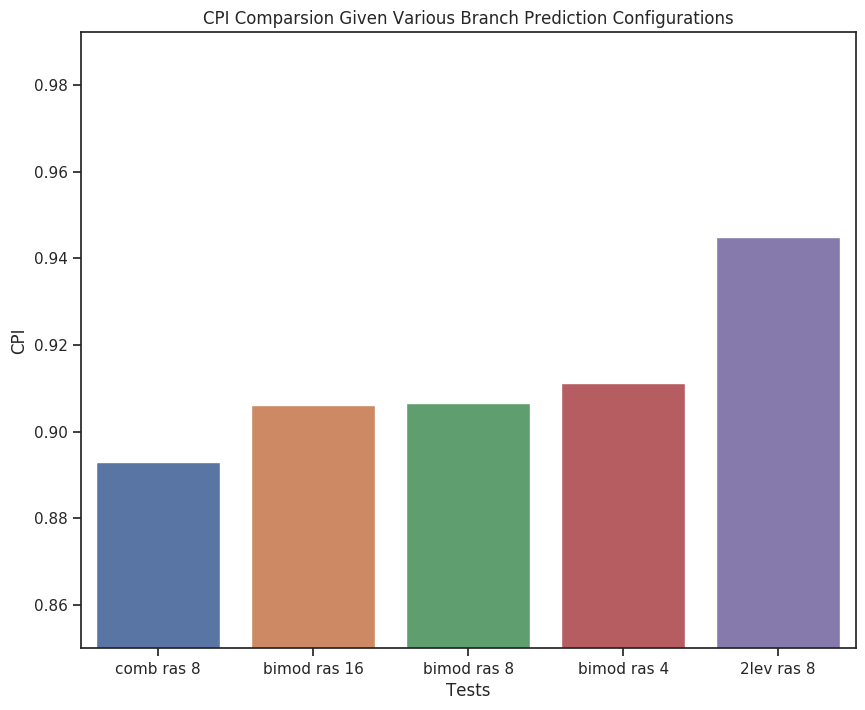
\includegraphics[width=0.68\columnwidth]{Lab-Tex/Lab9-images/cpi.png}
    \captionof{figure}{CPI comparison with varying branch prediction configurations}
    \label{fig:}
    \medskip
\endgroup

We know that the RAS is a tool used to make predictions for unconditional branches and jump instructions. It stores the predicted return address for an instruction so that the CPU does not have to stall to fetch this return address. \\

Given the bar graph above, we see that there is very little difference in CPI when varying the RAS with a bimodal prediction scheme. However, the values do show that a larger RAS results in a lower CPI. This is because a larger RAS means more return addresses can be saved and fewer overwrites happen. Although it seems that in this benchmark, there is little use of unconditional branches. The significant difference in CPI is found because of the prediction scheme. It seems that the combined scheme provides the best results, while the 2 level scheme is lacking.\\

The combined scheme providing the best CPI makes sense, as it selects for the prediction scheme that has historically performed well. If we assume that a certain chunk of the program/benchmark did well with the bimodal predictor, the combined scheme would initially select for this. However, once we move onto another chunk of the the program/benchmark, where the 2 level predictor does well, the combined scheme could select for the 2 level scheme. In this way, the combined scheme can be the best, despite the 2 level scheme being the worst, as it could be exploiting spatial locality.\\

\begingroup
    \centering
    \medskip
    %width=\columnwidth
    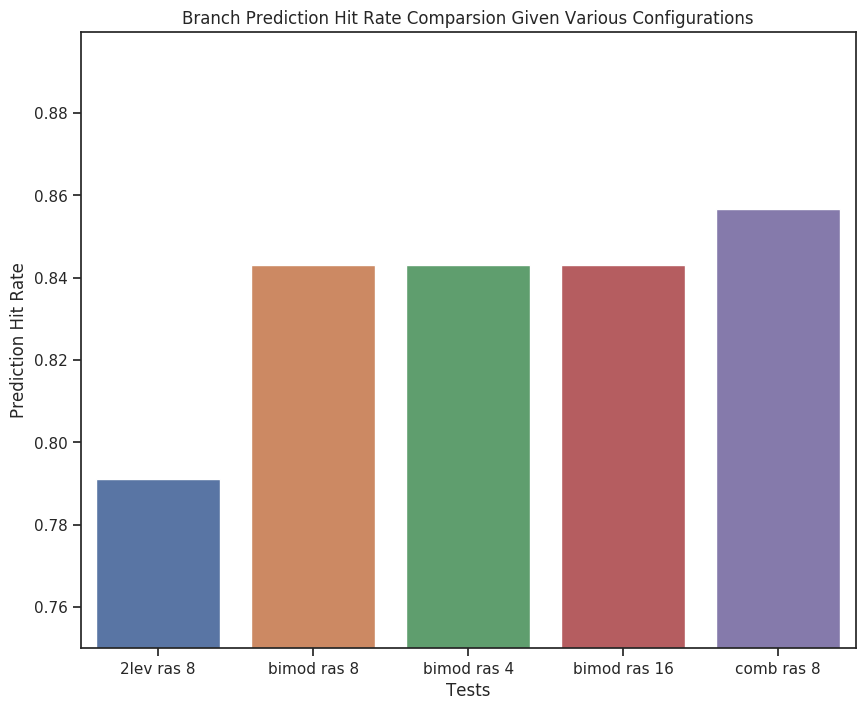
\includegraphics[width=0.68\columnwidth]{Lab-Tex/Lab9-images/hitRate.png}
    \captionof{figure}{CPI comparison with varying branch prediction configurations}
    \label{fig:}
    \medskip
\endgroup

Unsurprisingly, we see that the prediction rate is (almost) an inverse of the results of CPI. Although, there is no variation in prediction hit rate by increasing the RAS in the bimodal scheme. Once again, this is because the RAS works for unconditional branches, which almost always return to their intended address. Increasing the RAS size would have no effect on whether the prediction is correct or incorrect, unless a lot of overwriting in the RAS was happening, which does not seem like is the case. \\

\newpage

\section{BTB Configurations}

\begingroup
    \medskip
    \centering
    \def\arraystretch{1.5}
        \scriptsize{
        \begin{tabular}{cccccccc}
            \toprule
            Type & BTB Sets & BTB Assoc. & Address Hits & Address Misses\\
             \midrule
            bimod & 64 & 2 & 41812865 & 9234500\\
            \midrule
            bimod & 32 & 2 & 39367288 & 9234524\\
            bimod & 128 & 2 & 43872967 & 9234635\\
            \midrule
            bimod & 32 & 4 & 42186991 & 9234504\\
            bimod & 128 & 1 & 40873677 & 9234448\\
            \bottomrule
        \end{tabular}
        }
    \captionof{table}{Various configurations for branch prediction}
    \label{table:btb}
    \medskip
\endgroup


\begingroup
    \centering
    \medskip
    %width=\columnwidth
    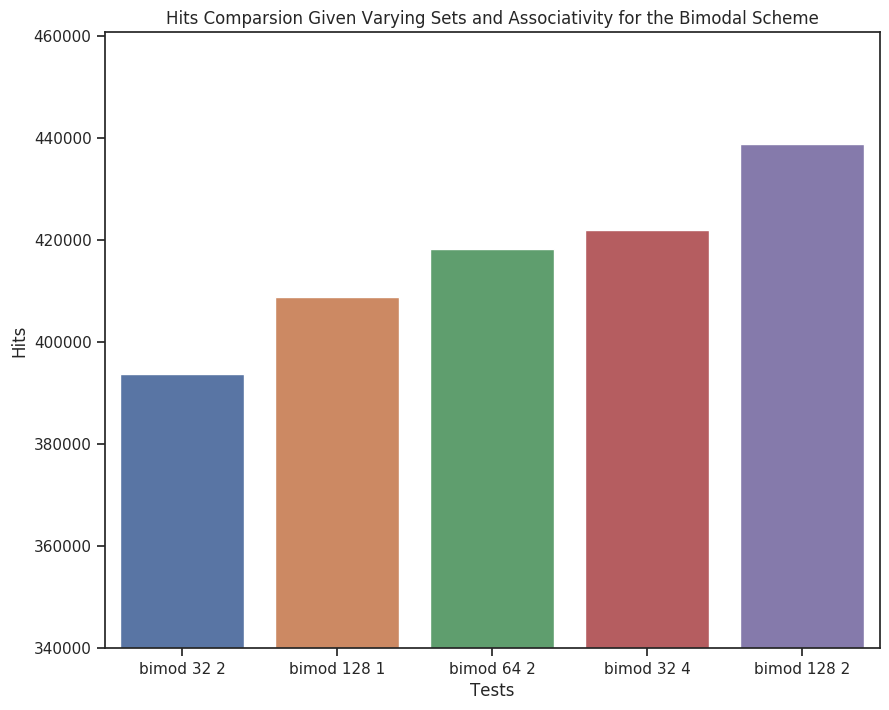
\includegraphics[width=0.68\columnwidth]{Lab-Tex/Lab9-images/hits_bimod.png}
    \captionof{figure}{Hits comparison with varying BTB configurations for the bimodal scheme}
    \label{fig:hits_bimodal}
    \medskip
\endgroup

Figure \ref{fig:hits_bimodal} indicates that increasing the associativity, given a fixed number of sets, increases the number of hits. We see that the 32/4 scheme outperforms the 32/2, while the 128/2 scheme outperforms the 128/1 scheme. Moreover, fixing the associativity, while increasing the number of sets, also provides a greater number of hits. \\

Moreover, a larger number of sets does not guarantee a higher number of hits. We see that the 64/2 scheme outperforms the 128/1 scheme, while the 32/4 scheme outperforms the 64/2 scheme. \\

Given the two observations above, it seems that having a larger BTB (sets x associativity) definitively results in more hits. The best performing scheme has 128*2 = 256 blocks, while the worst performing scheme has 32*2 = 64 blocks. The schemes in the middle have 128 blocks; interestingly, their hit rate does vary but with a lower significance in difference (empirically, the bar heights are closer). \\

Targeting the schemes with 128 blocks, we also see that a more "balanced" approach (decreasing sets and increasing associativity) tends to result in higher hits.\\

Putting all of this together, it is inferred that a 32/8 scheme would outperform the 128/2 scheme.

\begingroup
    \medskip
    \centering
    \def\arraystretch{1.5}
        \scriptsize{
        \begin{tabular}{cccccccc}
            \toprule
            Type & BTB Sets & BTB Assoc. & Address Hits & Address Misses\\
             \midrule
            bimod & 128 & 1 & 40873677 & 9234448\\
            bimod & 32 & 4 & 42186991 & 9234504\\
             \midrule
            bimod & 128 & 2 & 43872967 & 9234635\\
            bimod & 32 & 8 & \textbf{44708978} & 9234299\\
            \bottomrule
        \end{tabular}
        }
    \captionof{table}{Comparing the results of a 32/8 bimodal scheme to previous results}
    \label{table:infer}
    \medskip
\endgroup

Looking at Table \ref{table:infer}, it is indeed the case that 32/8 outperforms 128/2, despite both resulting in 256 blocks.\\

Just as with regular caches, we can determine that more entries results in more hits because there is more space to store predictions and reduce overwriting in the buffer. Similarly, increasing the associativity may improve performance because there are fewer collisions and overwrites
in the BTB. If instructions have the same last k bits, the BTB may be able to accomodate upto 8 of them at once before having to carry out replacement. Of course, it helps to have a larger cache. 

\begingroup
    \centering
    \medskip
    %width=\columnwidth
    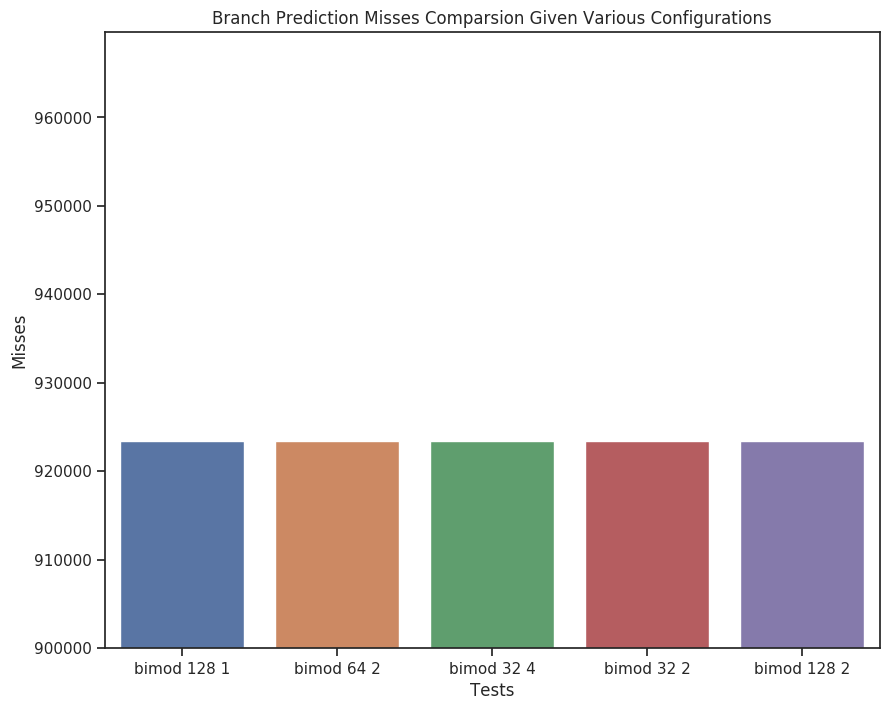
\includegraphics[width=0.68\columnwidth]{Lab-Tex/Lab9-images/misses_bimod.png}
    \captionof{figure}{Misses comparison amongst various BTB configurations for the bimod scheme}
    \label{fig:misses_bimod}
    \medskip
\endgroup

Looking at Figure \ref{fig:misses_bimod} and Table \ref{table:btb} shows that there is very little difference in misses amongst all the configurations. Moreover, there seems to be no immediately discernible pattern explaining whatever minor variance there exists. A potential theory is that misses refers specifically to those cases where a stored adddress was incorrect. Thus, in the case where there was no stored prediction for that instruction, it does not count towards a miss. That can explain why varying the buffer set and associativity does not change the number of misses.\\

The theory above was tested by changing the table size from 256 to 32, with a scheme of 64/2. However, there was a significant decrease in hits and increase in misses. \\

\section{Discussion and Conclusion}

For the latter section, it is quite unclear what the implications of setting a table size are, while varying the set and associativity. From the tests, it seems that the table size refers to a different entity than the BTB. The table size seems to be able to affect the hits and misses, while the BTB only affects the hits. 

Otherwise, relatively clear patterns emerge. For example, certain schemes clearly outperform others (combined has a lower CPI than 2 level). Further, increasing the product value of sets and associativity leads to more hits. 









%%%%%%%%%%%%%%%%%%%%%%%%%%5
% BIBLIOGRAFIA 
% Estilo de bibliografia ABNT. Se não tiver instalado, mude para plain ou ieeetr

%\bibliographystyle{plain} % Inclua isso se não tiver ABNTEX instalado
% \begin{thebibliography}{refs}
% \bibitem{}
\printbibliography
% \end{thebibliography}
\end{document}